\documentclass[xcolor=dvipsnames]{beamer}
\usetheme{Warsaw}

%\useoutertheme{infolines}
%\useinnertheme{circles}
\usepackage[utf8]{inputenc}
\usepackage{amsmath}
\usepackage{amsfonts}
\usepackage{amssymb}
% \usepackage{graphicx}
\usepackage{graphicx,epsfig}

\usepackage{textpos} 
\usepackage{listings}
\usepackage{hyperref}
\usepackage{multirow}
\usepackage{multicol}

\newcommand{\logoSENAC}{images/etec-small.png}
\newcommand{\logoUFSCar}{images/LogoUfscar.eps}
%\logo{\includegraphics[width=0.18\textwidth]{images/logoFATEC.png}\vspace{220pt}}


\setbeamertemplate{headline}{%
%\leavevmode%
%  \hbox{%
%    \begin{beamercolorbox}[wd=\paperwidth,ht=2.5ex,dp=1.125ex]{palette quaternary}%
%    \insertsectionnavigationhorizontal{\paperwidth}{}{\hskip0pt plus1filll}
%    \end{beamercolorbox}%
%  }

}

\addtobeamertemplate{frametitle}{}{%
	
	\small{
	
    \begin{textblock*}{\textwidth}(0cm,0.1cm)
		%\insertsectionnavigationhorizontal{\paperwidth}{}{\hskip0pt plus1filll}
%		\textcolor{gray}{\insertsectionhead\insertsubsectionhead}
		 
		
		%\insertsection \insertsubsection
    \end{textblock*}
	}
    




	% \begin{textblock*}{100mm}(0.93\textwidth,-0.55cm)
        % \includegraphics[width=0.15\textwidth]{\logoUFSCar}
    % \end{textblock*}




%    \begin{textblock*}{100mm}(0.93\textwidth,-0.75cm)
%        \includegraphics[width=0.1\textwidth]{\logoSENAC}
%    \end{textblock*}
}


\institute[]{
  %\inst{1}
  \includegraphics[width=0.25\textwidth]{\logoUFSCar}
} 

\setbeamercovered{transparent} 
\setbeamertemplate{navigation symbols}{} 
\setbeamercovered{invisible}




% \setbeamertemplate{footline}{% 
  % \hfill% 
  % \usebeamercolor[fg]{page number in head/foot}% 
  % \usebeamerfont{page number in head/foot}% 
  % \insertframenumber%
  % %\,/\,\inserttotalframenumber
  % \kern1em\vskip2pt% 
% }




% https://tex.stackexchange.com/questions/333587/beamer-frame-number-without-total/333684
\setbeamertemplate{footline}{
  \hfill%
  \usebeamercolor[fg]{page number in head/foot}%
  \usebeamerfont{page number in head/foot}%
  \insertframenumber%
  % \setbeamertemplate{page number in head/foot}[framenumber]%
  \usebeamertemplate*{page number in head/foot}\kern1em\vskip5pt%
}



%gets rid of bottom navigation bars
% \setbeamertemplate{footline}[frame number]{}
% \setbeamertemplate{footline}{\insertframenumber }



% \setbeamertemplate {footline}{\quad\hfill\insertframenumber\strut\quad}




% \setbeamertemplate{sidebar right}{}
% \setbeamertemplate{footline}{%
% \hfill\usebeamertemplate***{navigation symbols}
% \hspace{1cm}\insertframenumber{}}



% Define o caminho das figuras
\graphicspath{{images/}}

%\AtBeginSection[] 
%{
%    \begin{frame}
%	    \frametitle{Roteiro}
%	    \tableofcontents[currentsection]
%    \end{frame}
%}


%https://bloerg.net/2012/06/21/customizing-the-frametitle-of-beamer-presentation.html




\AtBeginSection[] 
{
    \begin{frame}
	    \frametitle{Roteiro}
	    \tableofcontents[currentsection]
    \end{frame}
}












%%%%%%%%%%%%%%%%%%%%%%%%%%%%%%%%%%%%%%%%%%%%%%%%%%%%%%%%%%%%%%%%%%%%%%%%%%%%%%%%%%%%
%%%%%%%%%%%%%%%%%%%%%%%%%%%%%%%%%%%%%%%%%%%%%%%%%%%%%%%%%%%%%%%%%%%%%%%%%%%%%%%%%%%%

\newcommand{\sumario}{
\begin{frame}[plain]
   \frametitle{Plano de Aula}
   \tableofcontents
\end{frame}
}

\newcommand{\frameTalkIsCheap}{
\begin{frame}{Exercícios}

	\addimage{images/talkischeap3}{0.65}{}

	\begin{flushright}
		Linus Torvalds
	\end{flushright}
\end{frame}		
}

\newcommand{\frameDuvidas}{
\begin{frame}{Dúvidas?}
	\addimage{images/questions.png}{0.65}{}
	 	
\end{frame}		
}


\newcommand{\addimage}[2]{
  \begin{figure}[!h]
  \centering
  \includegraphics[width=#2\paperwidth]{#1}
%  \caption{#3}
%  \label{fig:#4}
  \end{figure}
}


\newcommand{\addpdfpageh}[4]{
\includegraphics[trim={#1cm #2cm #1cm #2cm},clip,page=#4,height=0.8\paperheight]{#3}
}
\newcommand{\addpdfpagew}[4]{
\includegraphics[trim={#1cm #2cm #1cm #2cm},clip,page=#4,width=0.8\paperwidth]{#3}
}


%%%%%%%%%%%%%%%%%%%%%%%%%%
% blocks
%%%%%%%%%%%%%%%%%%%%%%%%%%

\newcommand{\popc}[2]{
\begin{block}{#1}
	\pause	
	#2
\end{block}
}

\newcommand{\pop}[2]{
\pause	
\begin{block}{#1}
	#2
\end{block}
}

\newcommand{\nblock}[2]{
\begin{block}{#1}
	#2
\end{block}
}

\newcommand{\eblock}[2]{
\begin{exampleblock}{#1}
	#2
\end{exampleblock}
}

\newcommand{\ablock}[2]{
\begin{alertblock}{#1}
	#2
\end{alertblock}
}



% Uma macro que cria \newenvironments
\newcommand{\coloredblock}[3]{
	\newenvironment{#1}[1]
	{
		\setbeamercolor{block title}{fg=white,bg=#2!75!black}%
		\begin{block}{#3}
	}
	{
		\end{block}
	}	
}

% Criaçao de \newenvironments
\coloredblock{blackblockenv}{black}{#1}
\coloredblock{blueblockenv}{blue}{#1}
\coloredblock{redblockenv}{red}{#1}

% Macro para chamar as \newenvironments criadas
\newcommand{\blackblock}[2]{
	\begin{blackblockenv}{#1}
		#2
	\end{blackblockenv}
}
\newcommand{\redblock}[2]{
	\begin{redblockenv}{#1}
		#2
	\end{redblockenv}
}
\newcommand{\blueblock}[2]{
	\begin{blueblockenv}{#1}
		#2
	\end{blueblockenv}
}









%\newcommand{\coloredblock}[3]{
%	\setbeamercolor{block title}{fg=white,bg=#1!75!black}%
%	\begin{block}{#2}
%		#3
%	\end{block}
%}
%
%\newcommand{\redblock}[2]{
%	\coloredblock{red}{#1}{#2}
%}
%
%\newcommand{\yblock}[2]{
%	\setbeamercolor{block title}{fg=white,bg=yellow!75!black}%
%	\begin{block}{#1}
%		#2
%	\end{block}
%}



%\newenvironment<>{myblock}[1]
%{%
%	\setbeamercolor{block title}{fg=white,bg=red!75!black}%
%	\begin{block}#2{#1}
%}
%{
%	\end{block}
%}
%  
%
%
%\newenvironment{blueblock}[1]
%{
%	\setbeamercolor{block title}{fg=white,bg=blue!75!black}%
%	\begin{block}{#1}
%}
%{
%	\end{block}
%}
%
%
%
%
%\newcommand{\mblock}[2]{
%\begin{block}{#1}
%	#2
%\end{block}
%}

%
%
%% Uma macro que cria \newenvironments
%\newcommand{\coloredblock}[3]{
%
%	\newenvironment{#1}[1]
%	{
%		\setbeamercolor{block title}{fg=white,bg=#2!75!black}%
%		\begin{block}{#3}
%	}
%	{
%		\end{block}
%	}
%	
%}
%
%% Criaçao de \newenvironment 
%\coloredblock{preto}{black}{#1}
%
%% Macro para chamar as \newenvironment criadas
%\newcommand{\blackblock}[2]{
%	\begin{preto}{#1}
%		#2
%	\end{preto}
%}

\author{Ovídio José Francisco\\
Orientadora: Prof.ª Dr. Katti Faceli\\
Coorientador: Prof. Dr. Rafael Geraldeli Rossi}
\title{Avaliação de Técnicas de Recuperação de Informação
para Organização e Extração de Conhecimento de Documentos de Reunião} 
\subtitle{}
% \date{\today} 
\subject{Dissertação de Mestrado} 


\begin{document}

\begin{frame}
	\titlepage
	 \begin{center}{}\end{center} 
\end{frame}
%\sumario

   \begin{frame}
		\frametitle{Roteiro}
		\tableofcontents
   \end{frame}

%\section{Introdução}
\section{Contextualização}



\begin{frame}{Contexto}

As atas registram assuntos discutidos em reuniões e podem ser utilizadas como base de dados.
\nblock{}{
\begin{itemize}
	\item Utilizadas como referência e apoio a decisões; 
	\item Um assunto pode ser discutido diversas vezes em reuniões diferentes;
	\item É desejável recuperar um histórico desses assuntos ao longo do tempo;
	\item Necessidade de ferramentas automáticas.
\end{itemize}
}

\end{frame}




\begin{frame}{Contexto}

Recuperação de Informação em documentos textuais:

\nblock{}{
\begin{itemize}
	\item Informações contidas em grandes quantidades de texto;
	\item Inerentemente não estruturados;
	\item Documentos com múltiplos assuntos;
	\item Assuntos dispersos pela base de documentos.
\end{itemize}
}

\end{frame}



\begin{frame}{Contexto}

% Um dos principais desafios nesse cenário é 
Nesse cenário, o desafio é encontrar trechos de texto que tratem somente do assunto pesquisado.

\nblock{}{

Essa tarefa consiste em 2 passos principais:
% Essa tarefa tem 2 passos principais:

\begin{itemize}
	\item Encontrar pontos onde há transição de assuntos;
	\item Identificar o teor desses assuntos;
\end{itemize}

} 

\end{frame}





\begin{frame}{Contexto}

Os algoritmos de segmentação textual são utilizados para dividir um texto em segmentos contendo um assunto completo e relativamente independente.

% \addimage{images/pre-process.png}{.9}{}

\nblock{}{
\begin{itemize}
	\item Úteis em aplicações com textos sem indicações de quebras de assunto, como transcrições de áudio, e diálogos em chats.
	\item Não dão indicações sobre o conteúdo dos segmentos.
\end{itemize}
} 

\end{frame}





\begin{frame}{Contexto}

% \nblock{}{
	% As técnicas de Extração de Tópicos são empregadas na organização de documentos.
	Os modelos de Extração de Tópicos podem estimar o assunto de cada documento de uma coleção.
	

% } 



\nblock{}{

\begin{itemize}
	\item Agrupam documentos por tópico.
	\item Identificam palavras para descrever o tópico do documento.
\end{itemize}
} 

\end{frame}







% ---------- Objetivos ----------
\section{Objetivos}
\begin{frame}{Objetivos}


\nblock{}{
	Propor uma solução para identificar, organizar e consultar assuntos registrados em atas de reunião.  
} 

\nblock{}{
	Utilizar técnicas de Segmentação textual em conjunto com modelos de Extração de Tópicos para:
	\begin{itemize}
	\item Gerar uma estrutura mais organizada que a coleção original.
	\item Utilizar a estrutura latente dos segmentos para Recuperação de Informação. 
	\end{itemize}
}
	% \item Dar início a investigação dessa abordagem no contexto de atas de reunião.


\end{frame}







% ---------- Proposta ----------
\section{Proposta}



\begin{frame}{Proposta}

	\center Visão Geral do Sistema.

	\addimage{images/visao-geral-3.eps}{.8}{}

\end{frame}


\begin{frame}{Proposta}

	\center Estrutura de dados interna e seu processo de geração.

	\addimage{images/estrutura.png}{.8}{}

\end{frame}


 
 
\begin{frame}{Proposta}

	\center Estrutura de dados interna e seu processo de geração.

	\begin{figure}[h!]

		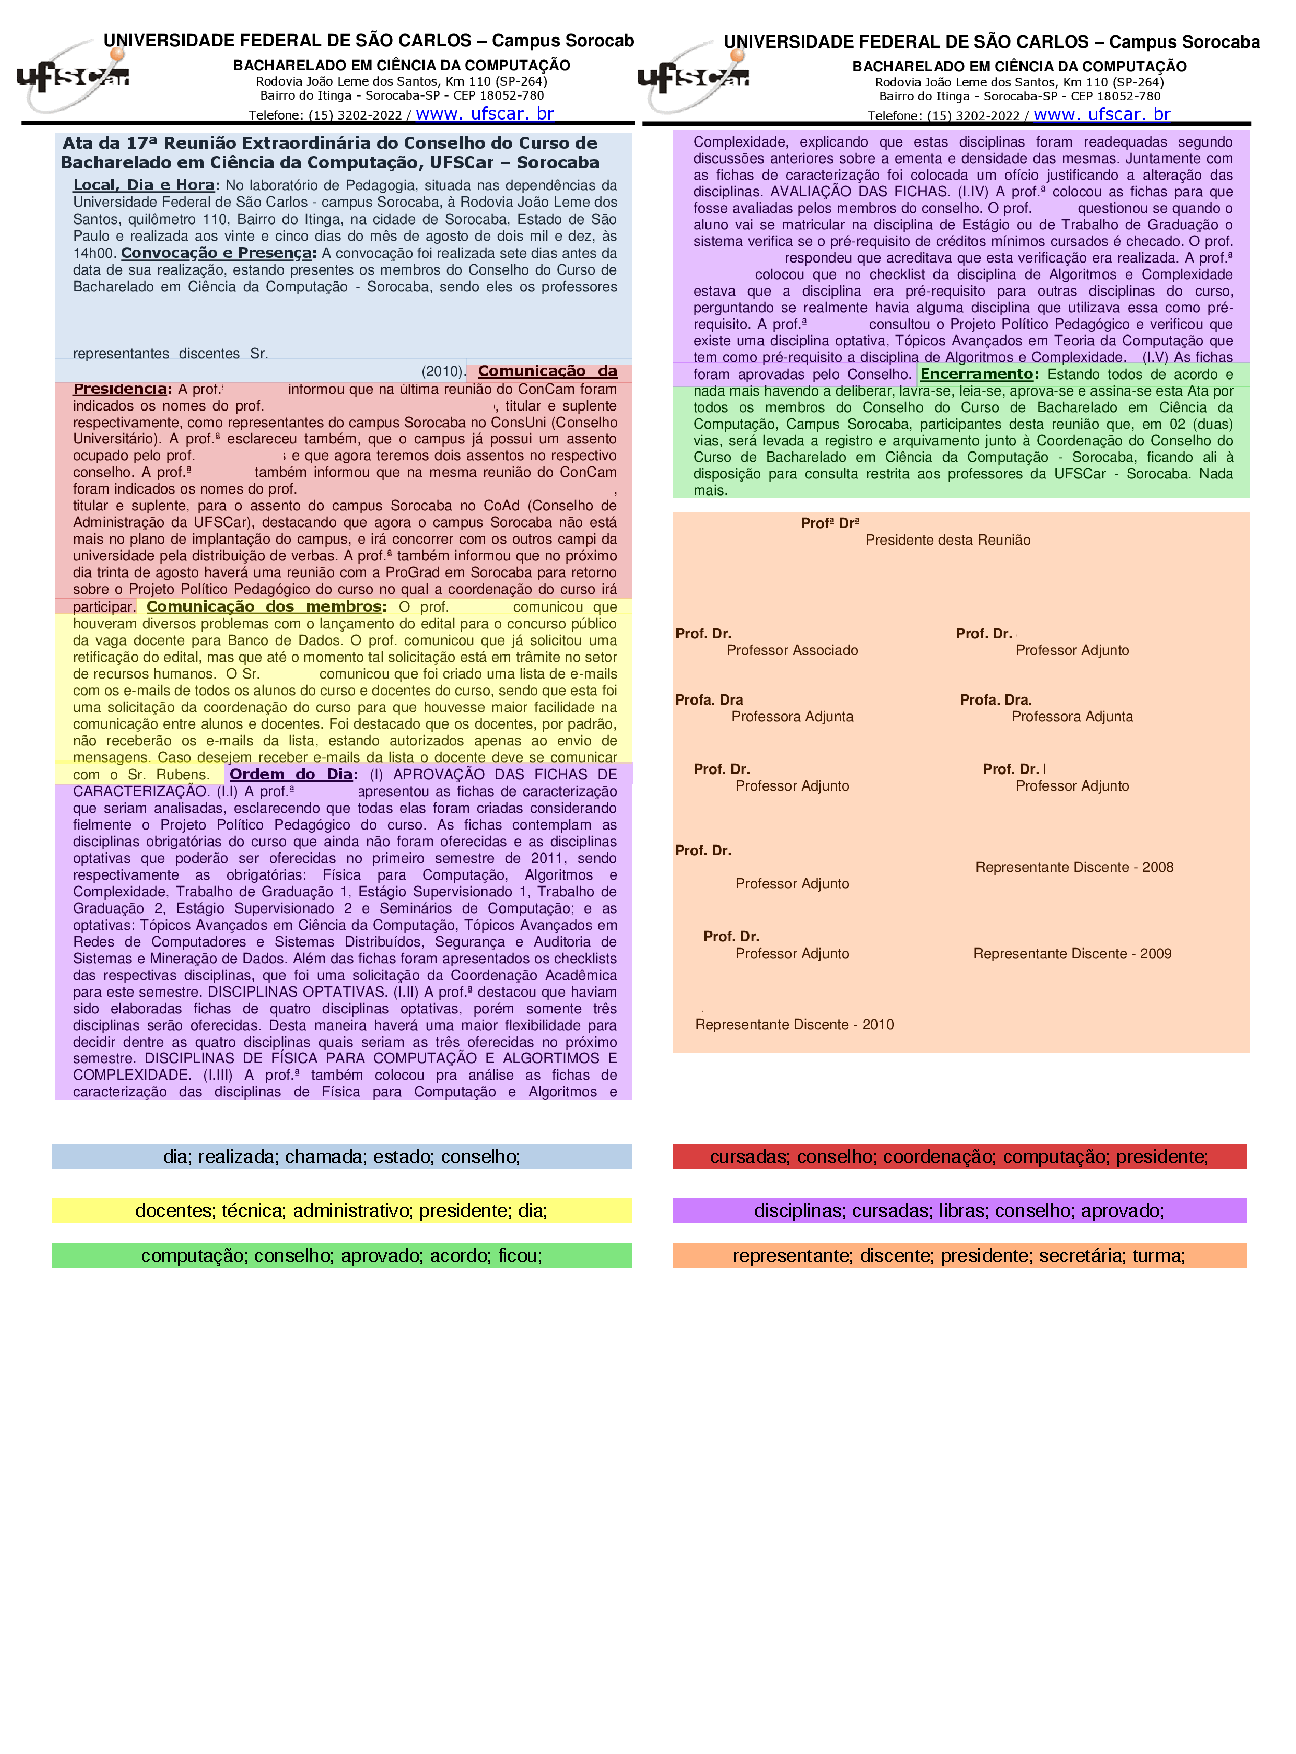
\includegraphics[trim={ 0 235 0 16 },clip,page=1,width=0.73\textwidth]{images/distribuicao.pdf}

	\end{figure}

\end{frame}

 
\begin{frame}{Proposta}
como os dados são apresentados?
- Tópico com maior similaridade com a consulta
	- MSV 

	(expansão de espaço?)

\end{frame}

 
 
% ---------- Análise dos Resultados ----------
\section{Análise dos Resultados}
\begin{frame}{Análise dos Resultados}




\begin{figure}[!h]
	\centering     %%% not \center
\tiny
	\subfigure[Ac]{ \label{fig:a}
		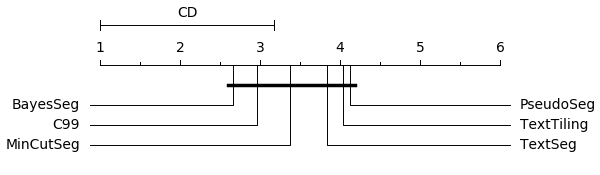
\includegraphics[width=47mm]{images/cds/Acuracia.png} 
	}	
	\subfigure[F^1]{ \label{fig:b}
		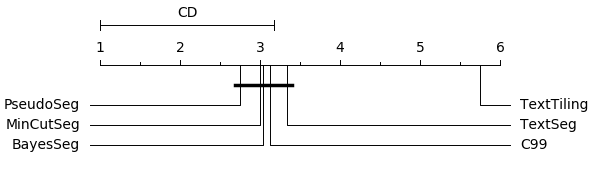
\includegraphics[width=47mm]{images/cds/F1.png} \\
	}
	\subfigure[P_k]{ \label{fig:c}
		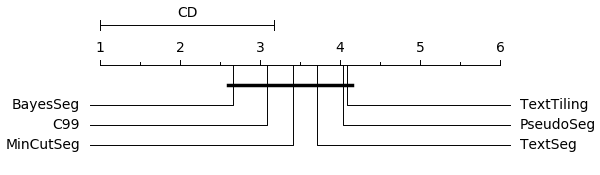
\includegraphics[width=47mm]{images/cds/Pk.png} 
	}
	\subfigure[WD]{ \label{fig:d}
		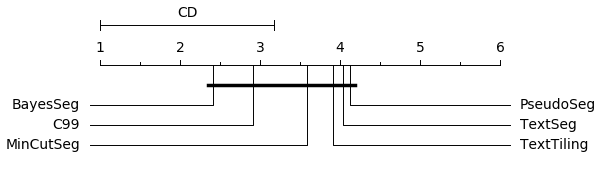
\includegraphics[width=47mm]{images/cds/WD.png} 
	}

		% \caption{Diagramas de Diferença Crítica sobre \textit{ranking} dos algoritmos de segmentação baseados em coesão léxica de acordo com valores de \textit{WindowDiff}, $P_k$, Acurácia, Precisão, Revocação e $F^1$.}
	% \label{fig:CDs}
\end{figure}
	
	
\end{frame}





% ---------- Conclusão ----------
\section{Conclusão}
\begin{frame}{Conclusão}
	
	
\end{frame}

% ---------- Trabalhos Futuros ----------
\begin{frame}{Trabalhos Futuros}
	
	
\end{frame}


\end{document}


%%%%%%%%%%%%%%%%%%%%%%%%%%%%%%%%%%%%%%%%%%%%%%%%%%%%%%%%%%
%%%%%%%%%%%%%%%%%%%%%%%%%%%%%%%%%%%%%%%%%%%%%%%%%%%%%%%%%%
%%%%%%%%%%%%%%% == FIM DA APRESENTAÇÃO == %%%%%%%%%%%%%%%%
%%%%%%%%%%%%%%%%%%%%%%%%%%%%%%%%%%%%%%%%%%%%%%%%%%%%%%%%%%
%%%%%%%%%%%%%%%%%%%%%%%%%%%%%%%%%%%%%%%%%%%%%%%%%%%%%%%%%%


\section{}
%%%%%%%%%%%%%%%%%%%%%%%%%%%%%%%%%%%%%%%%%%%%%%%%%%%%%%%%%%
\begin{frame}{}
	
	\nblock{}{
	
	}
	
\end{frame}
%%%%%%%%%%%%%%%%%%%%%%%%%%%%%%%%%%%%%%%%%%%%%%%%%%%%%%%%%%
	
